\chapter{Dependencies Between City Structure and Thermal Behaviour in Brno}
\label{app:Visualisation}

Long lasting heat waves bring about more severe living conditions in large urban environments. The phenomenon has been addressed mainly as urban heat islands (UHI). Determination of factors affecting UHI and good understanding of dependencies between city structure and thermal behaviour can significantly help municipalities in long-term strategic decision-making. A complex research effort using remote sensing techniques has been performed in the 2015. This appendix summarizes the preliminary results of the research, which is discussed in depth in \cite{NP16}. Let us note that TASI image data used for the OSTES testing in the Chapter \ref{chap:OSTESValid} were acquired within the scope of this research activity.

\section{Methods} 

The set of hyperspectral airborne data was collected in visible, near infrared, shortwave infrared and thermal infrared spectral regions using CASI, SASI and TASI sensors (ITRES, Canada), respectively. In addition to hyperspectral data, lidar mapping was performed using a Riegl 680i instrument (RIEGL, Austria). Taken together, these data have a high potential for providing valuable information relevant for modelling city thermal properties.

Data were acquired in both winter and summer days over the city of Brno, Czech Republic, both of which were climatologically extreme events. Winter acquisition was performed on 7th February 2015 at 21:53 (UTC). Summer acquisition was performed on 4th July 2015 at 14:03 (UTC) and at 20:59 (UTC). Complementary airborne laser scanning dataset was acquired on 22nd September 2015. The detailed description of data processing and study area is included in \cite{NP16}. 

The Figures \ref{fig:Transect1} and \ref{fig:Transect2} present the dependencies between city structure and city thermal regime. All displayed quantities are self explanatory except absorbed energy. This quantity relates surface absorptivity and solar irradiation accumulated during the daylight hours of 4th July 2015. Surface absorptivity was computed by subtracting surface reflectance from one. Then the surface absorptivity was multiplied by the direct plus diffuse solar irradiation, which was computed by SAGA Lighting and Visibility module (SAGA, 2013). The resulting quantity is absorbed energy by the surface.

\section{Results}

Results of visualisation are presented in the Figure \ref{fig:Transect1} and the Figure \ref{fig:Transect2}. Both figures have the following structure. The distance along the transect is represented by meters displayed on a horizontal axis. A true-colour composition from the CASI data is shown in the topmost panel. It contains yellow line indicating the transect along which were observed various quantities displayed in the following panels. Surface temperatures of a summer day and a summer night are shown in the second panel. Surface temperature of a winter night is shown in the third panel. A depiction of city structure is contained in the fourth panel. Digital terrain model (DTM) is shown in brown, while buildings are distinguished from high vegetation with grey and green colours, respectively. The Normalized Difference Vegetation Index (NDVI) is shown in the fifth panel and absorbed energy is shown in the last panel.

Several common observations can be made in both figures. The NDVI, as a measure of ``greenness'', follows a classification of high vegetation and also allows distinguishing between streets and a surfaces covered by grass. Local minima in absorbed energy follow shaded regions at the edges of buildings. Temperature over the areas covered by vegetation tends to be more stable and lower in average, while the temperature of streets and parking lots is significantly higher during summer day. We would like to point out several interesting features in the individual transects. These will be indicated by the distance in meters on the horizontal axis.

In Figure \ref{fig:Transect1} between 80 and 90 can be seen the stabilising role of vegetation – the temperature profile has a low variability as well as a lower average despite a higher amount of absorbed energy. In Figure \ref{fig:Transect1} at 305 and 390, two different roof surfaces can be observed – the rightmost one is dark, has a high absorptivity, while the leftmost one has a high reflectivity and reflects a cold sky in both summer and winter night. The region from 400 to 550 contains green areas which surrounds Špilberk castle. Summer day temperature is significantly lower in this region compared to other built up areas. The only notable temperature extreme is visible between 460 and 470 where the transect crosses a path walk.

The Figure \ref{fig:Transect2} shows interesting features as well. Roofs with high reflectivity can be observed at 160 – 170 and 530 – 540. The coldest places during a summer day are the river between 260 and 280 (which is on the other hand the warmest place in winter) and hard shadows next to high buildings, e.g. at 545. There is a notable shaded hillside between 40 and 50 causing temperature decrease in both summer day and night. There is an interesting dip in the summer night temperature profile between 360 and 370, which is presumably caused by a parked car in the parking lot. A dip in the summer temperature around 445 is caused by a roof window included in the transect.

\section{Conclusion}

The presented results show that hyperspectral image data with a high spatial resolution offers valuable information about the dependencies between the city structure and its thermal regime. Therefore the further analysis of these data should include quantification and modelling of various relations. 

\newpage
\begin{figure*}[!t]
\centering
\includegraphics[width=\linewidth]{pics/Appendix_B/Transect_1.pdf}
\vspace{1.5 em}
\caption{Visualisation of various characteristics through the transect, which reveal various dependencies between city structure and thermal regime of the Brno city. Detailed description of the quantities and image data can be found in the text.}
\label{fig:Transect1}
\end{figure*}

\newpage
\begin{figure*}[!t]
\centering
\includegraphics[width=\linewidth]{pics/Appendix_B/Transect_2.pdf}
\vspace{1.5 em}
\caption{Visualisation of various characteristics through the transect which reveal various dependencies between city structure and thermal regime of the Brno city. Detailed description of the quantities and image data can be found in the text.}
\label{fig:Transect2}
\end{figure*}

\end{appendices}